%\documentclass[notheorems]{beamer}
%\documentclass[handout]{beamer}
%\documentclass[handout,notes=show]{beamer}

\usetheme{metropolis}

\usepackage{amsmath, amssymb, amsfonts, tikz}
\usepackage[utf8]{inputenc}
\usepackage[T1]{fontenc}
\usepackage[english]{babel}

%\usepackage[default,osfigures,scale=0.95]{opensans}

\usepackage{fontspec}
\usefonttheme{professionalfonts} % using non standard fonts for beamer
\setsansfont[
Path           = /Users/alex/Library/Fonts/,
Extension      = .ttf,
Ligatures      = TeX,
UprightFont    = OpenSans-Light,
BoldFont       = OpenSans-Regular,
ItalicFont     = OpenSans-LightItalic,
BoldItalicFont = OpenSans-Italic
]{OpenSans}
\setmonofont[
Path           = /Users/alex/Library/Fonts/,
Extension      = .ttf,
Ligatures      = TeX,
UprightFont    = FiraCode-Regular,
ItalicFont    = FiraCode-Regular,
ItalicFont    = FiraCode-Regular,
]{DejaVu Sans Mono}
\metroset{block=fill}

% No navigation bars 
\beamertemplatenavigationsymbolsempty

\graphicspath{{img/}}

\definecolor{Purple}{HTML}{911146}
\definecolor{Orange}{HTML}{CF4A30}
\definecolor{Tan}{RGB}{225,221,191}
\definecolor{Green}{RGB}{76,131,122}
\definecolor{DB}{RGB}{4,37,58}

% Theme colors are derived from these two elements
\setbeamercolor{alerted text}{fg=Green}
\setbeamercolor{frametitle}{bg=Tan,fg=DB}
\usepackage{tabularx}
\usepackage{mathtools}
\usepackage{xmpmulti}
\usepackage{color}
\definecolor{keywordcolor}{rgb}{0.7, 0.1, 0.1}   % red
\definecolor{commentcolor}{rgb}{0.4, 0.4, 0.4}   % grey
\definecolor{symbolcolor}{rgb}{0.0, 0.1, 0.6}    % blue
\definecolor{sortcolor}{rgb}{0.1, 0.5, 0.1}      % green
\metroset{titleformat=smallcaps}


\newtheorem{proposition}[theorem]{Proposition}
\newtheorem{remarks}[theorem]{Remarks}
\newtheorem{remark}[theorem]{Remark}
\newtheorem{conjecture}[theorem]{Conjecture}


\theoremstyle{plain}
\newcommand{\terminology}[1]{\textbf{#1}}

\newcommand{\NN}{\mathbf{N}}
\newcommand{\ZZ}{\mathbf{Z}}
\newcommand{\QQ}{\mathbf Q}
\newcommand{\CC}{\mathbf C}
\newcommand{\RR}{\mathbf R}
\newcommand{\FF}{\mathbf F}
\newcommand{\lt}{<}
\newcommand{\gt}{>}
\newcommand{\amp}{&}
\newcommand{\diff}{\mathop{}\!\mathrm{d}}
\newcommand{\ints}{\mathcal{O}}
\newcommand{\ideal}[1]{\mathfrak{#1}}
\usepackage{mathrsfs}\usepackage{cancel}
\newcommand{\Gal}[2]{\operatorname{Gal}(#1/#2)}
\newcommand{\absgal}[1]{\operatorname{Gal}(\overline{#1}/#1)}
\DeclareMathOperator{\USp}{USp}
\DeclareMathOperator{\Spec}{Spec}

\newcommand{\sheaf}[1]{\operatorname{\mathcal{#1}}}
\newcommand{\inv}{^{-1}}
\DeclareMathOperator{\norm}{Nm}
\DeclareMathOperator{\ord}{ord}
\DeclareMathOperator{\divisor}{div}
\DeclareMathOperator{\PP}{\mathbf{P}}
\DeclareMathOperator{\Hom}{Hom}
\DeclareMathOperator{\Mat}{Mat}
\DeclareMathOperator{\End}{End}

\newcommand{\lb}{[}
\newcommand{\rb}{]}


\usepackage{listings}
\def\lstlanguagefiles{tex/lstlean.tex}

\lstset{language=lean,basicstyle=\ttfamily\scriptsize}

%\usepackage{mathfont}


\author{Alex J. Best (VU)}
\date{3/6/22 -- Intercity Seminar}
\title{Formalized number theory}
\subtitle{Past, present, and future}

\begin{document}

\begin{frame}
  \titlepage

  \note[item]{Thank the audience for being awake.}
\end{frame}

%\begin{frame}
%\frametitle{Table of Contents}
%\tableofcontents[currentsection]
%\end{frame}

\begin{frame}{In this talk}
    \begin{itemize}
        \item Past -- some results and areas that people have thought about in the past
        \item Present -- some current works in progress
        \item Future -- where we are going, what needs to be different to make progress
    \end{itemize}
    In number theory particularly, but also other areas of interest.
\end{frame}


\newcommand{\comment}[2]{#2}

\comment{

also cover importance of number theoretic algorithms

# Past
- Kepler - one big proof
- Elementary nt, via custom rings, pell etc
- Witt vectors
- Perfectoid spaces
- insolubility of the quintic in coq / lean,
- schemes in Lean (+ Isabelle too),
- some of the bits I did with Minkowski (also in HOL + isabelle),
- mason-stothers,
- basics of arith fns
- Lindemann-Weierstrass in coq
- ostrowski.
- prime number theorem
  - should be possible to "port" such a theorem to lean, but whats the point
- 1-dim diuedone

# Present 
## Some assorted smaller projects in mathlib
- David Loeffler adding Gamma function
- Kevin wilson density of squarefree numbers
- Michael Stoll, playing with hilbert symbols
- Antoine Chambert-Loir: Finite groups, simplicity of A_n's,
    A primitive subgroup of a permutation group \mathfrak S_nS
    n that contains a transposition is equal to \mathfrak S_nS
    n ; a primitive subgroup that contains a 3-cycle contains the alternating group.
  working from a group theory textbook Weilandt
  (maybe interesting to note that he was member of bourbaki until his 50th birthday in 2021,
  shortly thereafter started working more on some lean projects
- Alex kontorovich
- riccardo
- nuccio

- modular forms
- elliptic curves
- Sacha lean4, based on cohen, compare with, rings vs Z
- flt-regular, - mention computation of bernoulli in isabelle using...
- the unit fractions project,
- descent and the Sage bridge,
- adeles and statements of cft,
- p-adic L-functions
- Johan's talk

# Future
Issues / problems of interest
- Main issue is making the tools easier to use:
  - less verbose
  - tooling to catch common mistakes and problems, maybe even mathematically useful.
- writing at a level of detail closer to pen and paper maths, when the results are actually easy or standard in some way.
- how to speed up such 



I'd also like to mention some of the tooling / lintery things I wrote
and maybe find some nice instances where that's helped people.

I'd like to actually talk to a couple of people this week and find out
what they'd most like to hear, it's hard at this point to know what
people unfamiliar with the area are most interested in.
}

\begin{frame}{In the 2000s}
    Large projects such as the Kepler conjecture and the Odd order theorem.

    These were big collaborations with one main goal, and did involve some number theory adjacent topics.
    
    Now there is more of a trend to build on existing libraries to make more progress on deeper topics.
\end{frame}


%\begin{frame}{Lindemann-Weierstrass}
%    In Coq and Isabelle
%\end{frame}

\comment{
\begin{frame}[fragile]{pp}
\begin{lstlisting}
lemma fact_rec (n : ℕ) :
factorial (n + 1) = factorial n * (n+1) :=
begin
-- write out the definition of factorial
unfold factorial,
-- remember {1,...,n+1} = {1,...,n} ∪ {n+1}
rewrite list.range'_concat 1 n,
-- the product of two sequences joined together is just the product of the products of each sequence
rewrite list.prod_append,
-- I'm bored already are we done here?
simp,
-- YES!
end
\end{lstlisting}\pause

\end{frame}}


\begin{frame}{Perfectoids}
    Peter Scholze won a Fields medal in 2018 for ``transforming arithmetic algebraic geometry over $p$-adic fields through his introduction of perfectoid spaces, with application to Galois representations, and for the development of new cohomology theories.''
    \pause
    The definition is highly nontrivial, an unusual geometric object created from an extremely non-Noetherian ring.
    \pause

    \emph{In 2020ish} Kevin Buzzard, Johan Commelin, Patrick Massot  (building on others)  completed a long term project to define a perfectoid space formally in Lean.
\end{frame}

\begin{frame}{Perfectoids}
    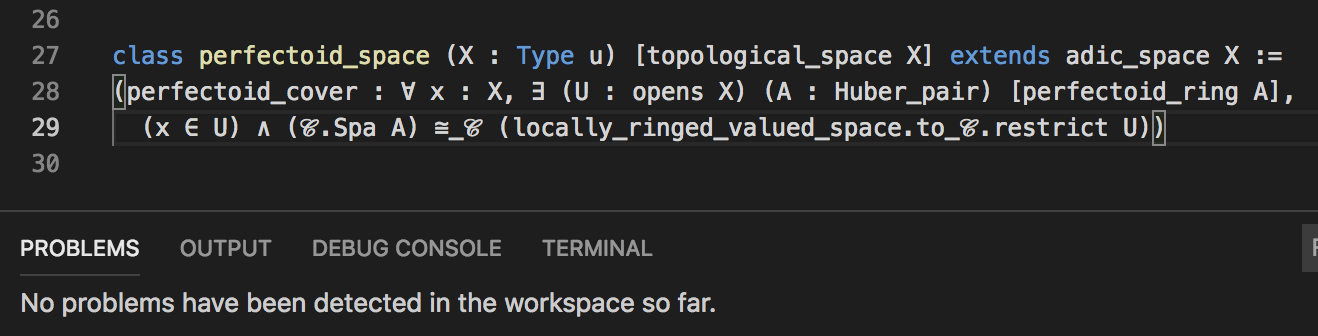
\includegraphics[width=\textwidth]{perfectoid.png}
    Lean has accepted the chain of definitions that lead to this are all valid, topological spaces, sheaves, valuations, adic spaces, perfectoid rings,...
    \pause

    It is difficult to estimate the amount of human effort expended to achieve this. \pause
    Their work relied on that of many others who are building \texttt{mathlib}, a general purpose library of mathematics from the ground up. \pause

    However, it also takes a long time for a human with no mathematical background to learn such a definition.
\end{frame}

\begin{frame}{One side effect: "new" algebraic structures}
    One ingredient of the theory surrounding perfectoid spaces (adic, spectral, Huber rings, etc.) is the notion of a valuation
    $$K \to \Gamma \cup \{0\}$$
    sending 0 to 0.

    In the course of the project the authors noticed they were having to repeat a lot of work on basic lemmas that were true both for fields and the value group above, inspired the creation of a new definition, a \emph{group with zero} (and monoid with zero, etc.).

    \begin{quote}
    ``Every sufficiently good analogy is yearning to become a functor.'' -- John Baez
    \end{quote}

    \begin{quote}
    Every sufficiently similar proof is yearning to become a new algebraic structure.
    \end{quote}
\end{frame}

\begin{frame}{Niche algebraic structures}
    There is even a lot of duplication between lemmas about groups, and those about groups with a zero.

    Earlier this year Yaël Dillies introduced a new algebraic structure, a division monoid, to be the correct setting for theorems, this is a monoid with an involutive inverse operation that doesn't always have $a \cdot a\inv  = 1$, but does have $a \cdot b = 1$ implies $a \inv = b$.

    \textbf{Upshot:} In order to formalize effectively and reduce duplication of effort generalizing proofs to unfamiliar algebraic structures is helpful.

\end{frame}

\begin{frame}{Generalizing theorems automatically}
    When we have so many algebraic structures, we don't want to spend our time trying to find the right structure to prove theorems in.

    Would prefer to write the proof under some assumptions we know work, and then let the proof \emph{assistant} tell us the most general and widely useful assumptions.
\pause
    \begin{lemma}
        Let $f\colon K\to L$ be a ring homomorphism between two fields, and $p$ be a natural number, then $K$ is characteristic $p$ if and only if $L$ is (including $p= 0$).
    \end{lemma}
\pause
    A Lean based tool I wrote last year will happily inform us that $K$ can be any division ring and $L$ can in fact be any nontrivial semiring.
   This works just by inspecting the original formalized proof.
\end{frame}

\begin{frame}{Backing up}
    Despite there being impressive progress on very advanced number theory, at least in the mathlib library there was not even the definition of a number field in Lean at the time

    Baanen, Dahmen, Ashvni Narayanan, Filippo Nuccio added Dedekind domains, and proved finiteness of the class group last year.

    Interestingly this formalization is uniform in the number field and function field cases, and avoids Minkowski's theorem in favour of simpler pigeonhole-type principles.

    But the basics of algebraic number theory are not really complete (Kummer-Dedekind, Kummer theory, Kronecker-Weber) in any formal system that I know.
\end{frame}

\begin{frame}{FLT-regular}
    In attempt to fill the gaps and add more down-to-earth algebraic number theory we have started a project to formalize Kummer's proof of Fermat's last theorem for regular primes
    $$p \nmid h_{\QQ(\zeta_p)}$$
    this splits into two cases for
    $$x^p + y^p = z^p$$

    Case I: $p\nmid xyz$ (comparatively elementary, lots of progress, computing basics about cyclotomic fields, ...)

    Case II: $p\mid xyz$ (requires some class field theory in an essential way, even on paper the proofs are long)
\end{frame}

\begin{frame}{Some progress}
    María Inés de Frutos Fernández has formalized the ring of Adèles (and Idèles) and given the \emph{statement} of the main theorem of global CFT in Lean:
    \begin{theorem}
        Let $K$ be a number field. Denote by $C_{K}^{1}$ the quotient of $C_{K}$ by the connected component of the identity. There is an isomorphism of topological groups $C_{K}^{1} \simeq G_{K}^{a b}$.
    \end{theorem}
    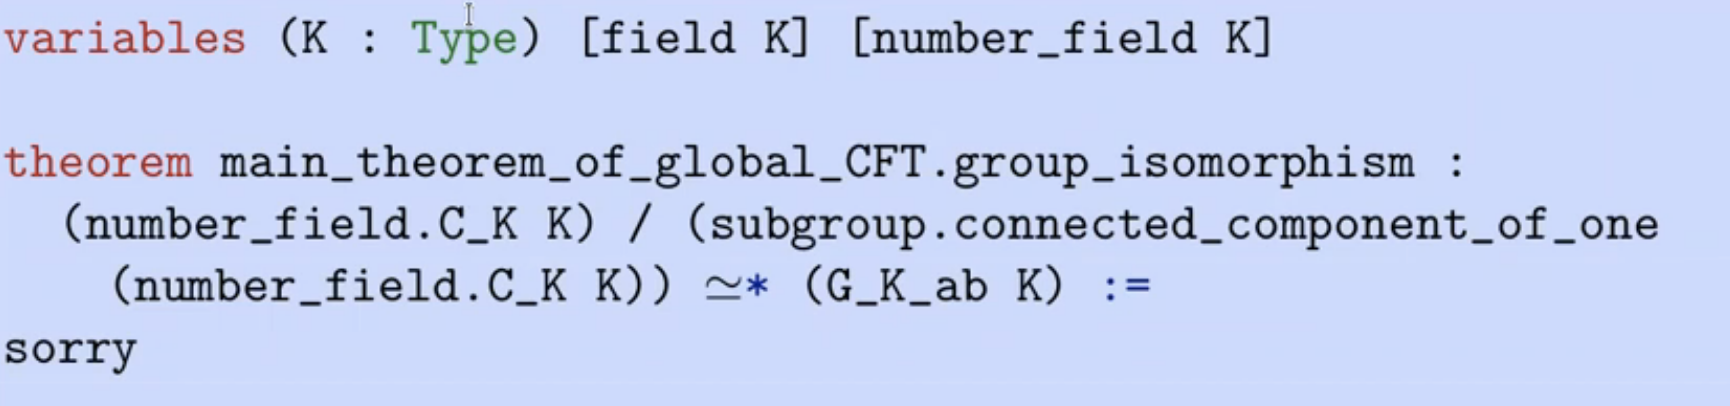
\includegraphics[width=\textwidth]{maria.png}
\end{frame}

\begin{frame}{Descent}
    With Anne Baanen, Nirvana Coppola, Sander Dahmen, we have been formalizing some Mordell-style descent to find integral points on elliptic curves: for example the non-existence of integral points on
    $$y^2 = x^3 - 5$$\pause
    Basically works, except, we still need to compute the class group of $\QQ(\sqrt{-5})$!

    This sort of proof necessarily involves some amount of hands on calculation, this is often harder to formalize than clean theory. % Part of this is due to implicit normal forms in the way we think about elements of number fields, writing everything formally in terms of a basis is annoying!

    In order to work conveniently with such calculations we have added tactics to handle calculations in rings with a finite ``multiplication table'' automatically, and write formal proofs that aren't significantly longer than paper ones.

    The other strategy is to leverage existing computer algebra systems where possible but still checking the output.
\end{frame}

\begin{frame}{Certifying number theoretic computations}
    Eventually would be helpful to have code that computes class groups implemented in a formal system.

    Right now this is a lot of work repeating the excellent pre-existing algorithms in a new language.  \pause

    \textbf{Question:} Is it possible to compute the class group with a computer algebra system (e.g. Sage), and write down a certificate of the result that is easily checkable (fast to check, not too long, and mathematically simple!)

    Ideally the certificate would be a text file, other users shouldn't need to install the CAS to repeat the calculation, but it should be provable in the system.

    But the certification itself should not rely on GRH etc.
\end{frame}

\begin{frame}{The Hasse Norm theorem}
    Suppose we want to check that an explicitly given ideal in a number field is non-principal, can we give a certificate for this.

    One idea: If an ideal is principal, it's norm must be equal to the norm of an element (and this holds everywhere locally too).

    \begin{theorem}[Hasse Norm theorem]
        If $K/\mathbf Q$ is a cyclic Galois extension and $x \in \mathbf Q$ is everywhere locally a norm, then $x$ is globally a norm.
    \end{theorem}
\pause
    There are counterexamples to this in the biquadratic case due to Hasse (and Serre-Tate) (and for any non-cyclic case Frei, Loughran, Newton).

    Number fields for which this property holds are said to satisfy the \emph{Hasse norm principle}.
\end{frame}

\begin{frame}{The Hasse Norm theorem}
    \begin{theorem}[Frei, Loughran, Newton]
        Let $k$ be a number field and $G$ a finite abelian group. Then 100\% of $G$-extensions of $k$, ordered by conductor, satisfy the Hasse norm principle.
    \end{theorem}\pause
    But if we order by discriminant:

    \begin{theorem}[Frei, Loughran, Newton] Let $G$ be a non-trivial finite abelian group and let $Q$ be the smallest prime dividing $|G|$. Assume that $G$ is not isomorphic to a group of the form $\mathbb{Z} / n \mathbb{Z} \oplus(\mathbb{Z} / Q \mathbb{Z})^{r}$ for any $n$ divisible by $Q$ and $r \geq 0$. Then a positive proportion of $G$-extensions of $k$ fail the Hasse norm principle, ordered by discriminant.
    \end{theorem}
    So locally verifying non-principality might be viable for abelian number fields.
\end{frame}

\begin{frame}{Other ideas}
    There are many useful algorithms with "obvious" certificates:
    \begin{itemize}
        \item Ideal membership
        \item Matrix normal forms (SNF, HNF, LU, RREF)
        \item Factoring
        \item Checking solubility modulo primes
    \end{itemize}
\pause
    Have a tool that talks to Sage to certify some of these in Lean already, working on others.

    I'd be happy to learn of other instances of this pattern!

    This might be independently a nice check for CASes, when further advanced.
\end{frame}

%\begin{frame}{Implementing number theoretic algorithms}
%\end{frame}

\begin{frame}{Implementing number theoretic algorithms}
    Alternatively we can implement algorithms within a proof assistant, as efficient functions that give the same output as what we want to compute
    \begin{itemize}
        \item Gives us a guaranteed correct implementation.
        \item We can experiment with modifying / improving the algorithm, and prove correctness or equality with the original one.
        \item We can prove properties, or "run" the algorithm in families, in ways normal code can't.
    \end{itemize}

    After writing the algorithm down, it is only accepted as a genuine mathematical function when it is shown to halt.
    With some functions this is obvious, but for algorithms that use recursion or unbounded loops, less so!
\end{frame}

\begin{frame}{Tate's algorithm}
    Sacha Huriot-Tattegrain (+B.+Dahmen) has implemented Tate's algorithm in Lean(4).

    \begin{itemize}
        \item Complete algorithm to compute local invariants of an elliptic curve, including the $c_p(E), \ord_p(\Delta_E), \ord_p(N_E)$

        \item Works in characteristic 2 and 3.

        \item Based on Cohen's description of the algorithm, but at times consulting other sources and even the GP source code was necessary to get it right.

        \item It runs fast!

        \item Partly generalized to base rings beyond $\ZZ$.
    \end{itemize}

    Without an independent definition of the Kodaira types and conductor exponent we cannot actually check the algorithm does what it says.
    Nevertheless we could prove certain properties of the algorithm in future, such as invariance under change of the initial model.
\end{frame}


\begin{frame}{Unit fractions}
    In December 2021 Thomas Bloom posted a paper: On a Density Conjecture about Unit Fractions to arXiv (2112.03726)
    \begin{quote}
        \mathbf{Abstract:} We prove that any set $A \subset \mathbb{N}$ of positive upper density contains a finite $S \subset A$ such that $\sum_{n \in S} \frac{1}{n}=1$, answering a question of Erdős and Graham.
    \end{quote}
    18 pages, quickly recognized as correct and widely applauded in popular press (Quanta, etc), generalizes an older result of Croot.

    Thomas Bloom and Bhavik Mehta are working hard to formalize the paper.
\end{frame}

\begin{frame}
    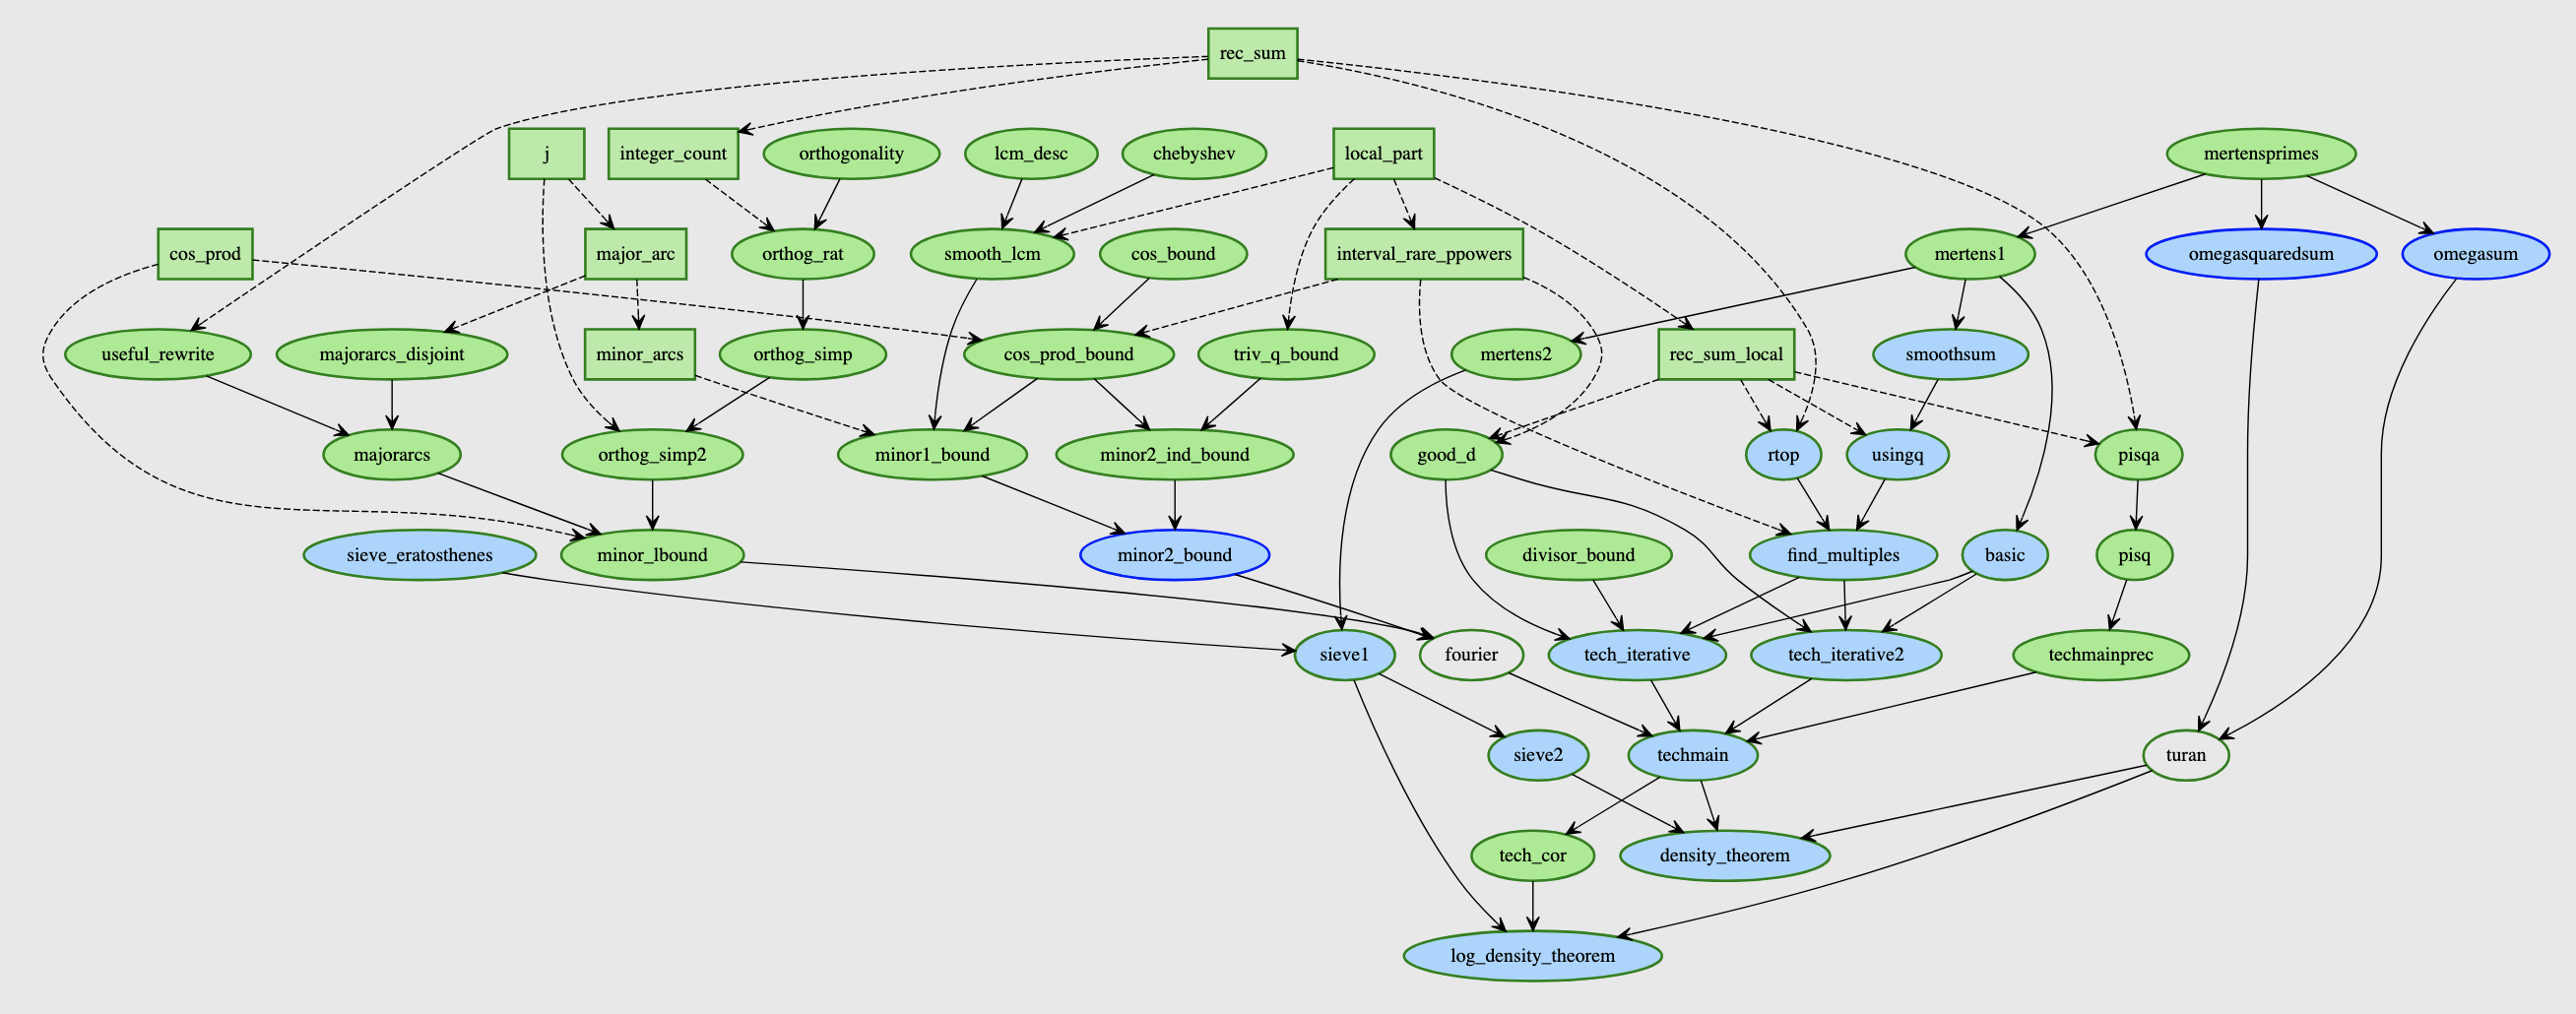
\includegraphics[width=1.1\linewidth]{unit.png}

    Many nice outputs from this project for analytic number theory and density results too.
\end{frame}

\begin{frame}{Collaboration Galore}
    One nice aspect of formalization is community, we are building on each others work, but the gaps have to line up precisely.

    This both eases collaboration (I can not worry about the details of your proof if it compiles and I understand the statement), but it also makes it harder, I have to contend and work with the community agreed upon definition of an object, rather than make my own variant.

    Nevertheless working on such a library has the feeling of collaborating on a large textbook / reference work.
\end{frame}

\begin{frame}{Collaboration Galore}
    \begin{itemize}
        \item Chris Birkbeck: Defining modular forms + Eisenstein series (like Manuel!)
        \item David Loeffler: Defining the Gamma function, analytic continuation
        \item Antoine Chambert-Loir: Finite groups, simplicity of $A_n$'s
        \item Amelia Livingston: Group cohomology
        \item Brandon H. Gomes and Alex Kontorovich: statement of the Riemann Hypothesis
        \item Michael Stoll: re-doing Legendre symbols, proved Hilbert reciprocity for quadratic Hilbert symbols over $\QQ$
        \item Sophie Bernard \& Cyril Cohen \& Assia Mahboubi \& Pierre-Yves Strub, and Thomas Browning: Insolvability of General Higher Degree Equations
        \item Kevin Wilson: calculation of the density of squarefree numbers as $\zeta (2)\inv = 6 / \pi ^2 $.
    \end{itemize}
\end{frame}

\begin{frame}{Closing thoughts}
    Formalization of mathematics (including number theory) is still slow and painful at times.

    But we have several thousand years of mathematics, and learning how to think about, and explain mathematics, to catch up on.

    Thinking about these issues and finding clean arguments can be a lot of fun, and the tool may occasionally surprise you.
\end{frame}


\comment{








\begin{frame}{Some examples: Grunwald(-Wang) and K-theory}

    \begin{quotation}
        Some days later I was with Artin in his office when Wang appeared. He said he had a counterexample to a lemma which had been used in the proof. An hour or two later, he produced a counterexample to the theorem itself... Of course he [Artin] was astonished, as were all of us students, that a famous theorem with two published proofs, one of which we had all heard in the seminar without our noticing anything, could be wrong.

        --- Tate
    \end{quotation}\pause

    \note{The problem: 2, the cursed prime. This is often an edge case.}

    \begin{quotation}
        The groundbreaking 1986 paper “Algebraic Cycles and Higher K-theory” by Spencer Bloch was soon after publication found by Andrei Suslin to contain a mistake in the proof of Lemma 1.1. The proof could not be fixed.

        --- Voevodsky
    \end{quotation}

\end{frame}

\begin{frame}{The solution: Take 2}
    What if computers could do the boring work for us?\pause

    Computers are:
    \begin{itemize}
        \item Capable of checking basic logical statements,\pause
        \item Fast,\pause
        \item Never complain.
    \end{itemize}
\end{frame}

\begin{frame}{The new problem}
    How do you describe the steps of a proof to a computer with as little pain as possible? \pause
    Often mathematicians leave unsaid many steps which are intuitive or easily supplied. \note{(this is one place mistakes enter)}\pause

    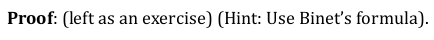
\includegraphics[height=2em]{pf-exercise.png}\pause

    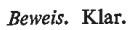
\includegraphics[height=1.5em]{beweis-klar.png}\pause

    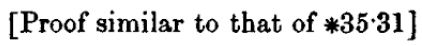
\includegraphics[height=1.5em]{pf-similar.png}\pause

    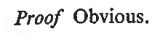
\includegraphics[height=2em]{pf-obvious.png}\pause

    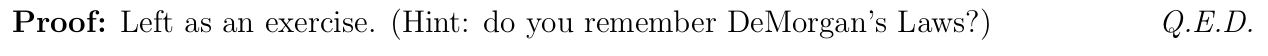
\includegraphics[height=1.5em]{pf-remember.png}\pause

    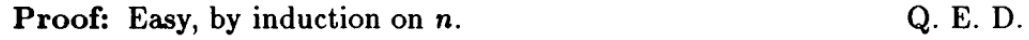
\includegraphics[height=1.1em]{pf-easy-induct.png}\pause

    The computer will probably not understand these, but in order to stay sane we must strike a balance between detail and verbosity.\note{ Teach the computer to work off as little as possible.}
\end{frame}

\begin{frame}{Enter Lean}
    The idea of trying this sort of thing has been around for a while. \pause

    But only within the last few years has it begun to seem more feasible for an average mathematician to do this. Tools have gotten better, slowly this idea has gained traction.\pause

    Recently an interactive proof assistant called Lean has been under heavy development. And I've been playing with it.

    Let me show you some lean code:
\end{frame}

\begin{frame}[fragile]
\begin{lstlisting}
lemma fact_rec (n : ℕ) :
factorial (n + 1) = factorial n * (n+1) :=
begin
-- write out the definition of factorial
unfold factorial,
-- remember {1,...,n+1} = {1,...,n} ∪ {n+1}
rewrite list.range'_concat 1 n,
-- the product of two sequences joined together is just the product of the products of each sequence
rewrite list.prod_append,
-- I'm bored already are we done here?
simp,
-- YES!
end
\end{lstlisting}\pause
We can replace all of the above with: \lstinline{by unfold factorial; simp [list.range'_concat, list.prod_append]}
\note{ Lean will figure out when and how to apply the lemmas.}

\end{frame}

\begin{frame}{(not so?) Live demo!}
    \multiinclude[<+->][format=png, graphics={width=\textwidth}]{fact}
\end{frame}

\begin{frame}{But can it do research?}
    Research level mathematics requires a vast body of knowledge to even think about.
    \pause

    As humans we forget this and also gloss over things we (think we) know well.
    \pause

    For instance one can forget what a Dedekind cut is, or Peano arithmetic and still think about real and natural numbers without an issue.
    Our intuition allows us to abstract these concepts so far away that we don't have to work from the ground up when approaching a problem.

\end{frame}}

\end{document}
